\documentclass[11pt,twoside,a4paper]{article}
% http://www-h.eng.cam.ac.uk/help/tpl/textprocessing/latex_maths+pix/node6.html symboles de math
% http://fr.wikibooks.org/wiki/Programmation_LaTeX Programmation latex (wikibook)
%=========================== En-Tete =================================
%--- Insertion de paquetages (optionnel) ---
\usepackage[french]{babel}   % pour dire que le texte est en fran{\'e}ais
\usepackage{a4}	             % pour la taille   
\usepackage[T1]{fontenc}     % pour les font postscript
\usepackage{epsfig}          % pour gerer les images
%\usepackage{psfig}
\usepackage{amsmath, amsthm} % tres bon mode mathematique
\usepackage{amsfonts,amssymb}% permet la definition des ensembles
\usepackage{float}           % pour le placement des figure
\usepackage{verbatim}

\usepackage{longtable} % pour les tableaux de plusieurs pages

\usepackage[table]{xcolor} % couleur de fond des cellules de tableaux

\usepackage{lastpage}

% \usepackage[top=1.5cm, bottom=1.5cm, left=1.5cm, right=1.5cm]{geometry}
% gauche, haut, droite, bas, entete, ente2txt, pied, txt2pied
\usepackage{vmargin}
\setmarginsrb{1.0cm}{1.0cm}{1.0cm}{1.0cm}{15pt}{3pt}{90pt}{3pt}

\usepackage{lscape} % changement orientation page
%\usepackage{frbib} % enlever pour obtenir references en anglais
% --- style de page (pour les en-tete) ---
\pagestyle{headings}

% % % en-tete et pieds de page configurables : fancyhdr.sty

% http://www.trustonme.net/didactels/250.html

% http://ww3.ac-poitiers.fr/math/tex/pratique/entete/entete.htm
% http://www.ctan.org/tex-archive/macros/latex/contrib/fancyhdr/fancyhdr.pdf
\usepackage{fancyhdr}
\pagestyle{fancy}
% \newcommand{\chaptermark}[1]{\markboth{#1}{}}
% \newcommand{\sectionmark}[1]{\markright{\thesection\ #1}}
\fancyhf{}
\fancyhead[LE,RO]{\bfseries\thepage}
\fancyhead[LO]{\bfseries\rightmark}
\fancyhead[RE]{\bfseries\leftmark}
\fancyfoot[LE]{\thepage /\pageref{LastPage} \hfill
	Matrix Query Language (MQL) -- \emph{Confidentiel *****}
\hfill 
\includegraphics[width=0.5cm]{img/logo_glider.png} }
\fancyfoot[RO]{
\includegraphics[width=0.5cm]{img/logo_glider.png} \hfill
	\emph{Confidentiel *****} -- Matrix Query Language (MQL)
\hfill \thepage /\pageref{LastPage}}
\renewcommand{\headrulewidth}{0.5pt}
\renewcommand{\footrulewidth}{0.5pt}
\addtolength{\headheight}{0.5pt}
\fancypagestyle{plain}{
	\fancyhead{}
	\renewcommand{\headrulewidth}{0pt}
}

\renewcommand{\headrulewidth}{0.25pt}
\renewcommand{\footrulewidth}{0.5pt}
%% \setlength{\headheight}{85pt}
% \addtolength{\headheight}{0.5pt}
% \fancypagestyle{plain}{
% 	\fancyhead{}
% 	\fancyfoot{}
% 	\renewcommand{\headrulewidth}{0pt}
% }

%--- Definitions de nouvelles commandes ---
\newcommand{\N}{\mathbb{N}} % les entiers naturels


%--- Pour le titre ---
\def\maketitle{%
	\begin{center}
		\begin{tabular}[c]{c|c}
			\textsc{\textbf{Institution}}~\\[\baselineskip]~\\[\baselineskip]
			\emph{\textbf{Date 09-09-2009}}~\\[\baselineskip]~\\[\baselineskip]
			\emph{\textbf{Pr{\'e}cisions relatives au contexte}}~\\[\baselineskip]~\\[\baselineskip]
			\textsc{Auteur inestimable}~\\[\baselineskip]~\\[\baselineskip]
			& 
			
\includegraphics[width=3cm]{img/logo_glider.png}~\\[\baselineskip]
		\end{tabular}
		% \\ \hline
		 	% % if more than one logo
			% 
\includegraphics[width=5cm]{img/logo_glider.png}
			% 
\includegraphics[width=5cm]{img/logo_wifi.png}
		% \\ \hline
		% \end{tabular}
			~\\[\baselineskip]~\\[\baselineskip]
			\Huge{Titre principal}~\\[\baselineskip]
			\Large{Titre secondaire}~\\[\baselineskip]
		
		~\\[\baselineskip]
		~\\[\baselineskip]
	\large{
		\textsc{\textbf{Institution d'accueil et jury}}
		~\\[\baselineskip]
		<<titre personne>> : \texttt{Anne ONYME}~\\[\baselineskip]
		<<titre personne>> : \texttt{Jocelyn CONNU}~\\[\baselineskip]
		~\\[\baselineskip]
		\textit{Pr{\'e}cisions du contexte de r{\'e}daction de l'article}
	}

	\end{center}

}%



%--- Pour le glossaire --- a defaut de \makeglossary ou d'utilisation d'index latex

\definecolor{verylightgray}{rgb}{0.8,0.8,0.8}
\def\makeglossaire{%
	\begin{center}

	\begin{tabular}{|>{\columncolor{verylightgray}} p{0.2\textwidth}|p{0.8\textwidth}|}

		\hline

		\textbf{BLAST} & 

			\begin{tabular}{p{0.8\textwidth}}

			Basic Local Alignment Search Tool \\

			\textit{algorithmes et logiciels pour l'alignement de s{\'e}quences et la recherche de similarit{\'e}s locales}

			\end{tabular} \\

		\hline

		\textbf{BNDB} & Biochemical NetWork DataBase \textit{(entrep{\^o}t de donn{\'e}es)} \\

		\hline

	\end{tabular}

\end{center}

}%

%============================= Corps =================================
\begin{document}

%% %ecrire le titre...
%% \maketitle
%% \setcounter{page}{0}
%% \thispagestyle{empty}
%% \clearpage
%% \setcounter{page}{0}
%% \thispagestyle{empty}
%% ~\\
%% \clearpage
%% \setcounter{page}{0}
%% \thispagestyle{empty}
%% % ecrire la table des mati{\'e}res...
%% \tableofcontents
%% % \clearpage
%% % \setcounter{page}{0}
%% % \thispagestyle{empty}
%% % ecrire la table des figures et celle des tableaux
%% \setcounter{page}{0}
%% \thispagestyle{empty}
%% ~\\ \rule{10cm}{1mm}~\\
%% \listoffigures
%% ~\\ \rule{10cm}{1mm}~\\
%% \listoftables
%% \clearpage

\setcounter{page}{1}

\texttt{http://enoviaplmtutors.blogspot.fr/2012/11/query-languagemql-mql-command-editor.html}

\section*{Matrix Query Language\markboth{Matrix Query Language}{Matrix Query Language}}
\addcontentsline{toc}{section}{Matrix Query Language}

\subsection*{What is MQL?\markboth{What is MQL?}{What is MQL?}}
\addcontentsline{toc}{subsection}{What is MQL?}

MQL stands for Matrix Query Language it is just Similar to SQL, MQL which consists of a set of statements. Query, build, instantiate and maintaina a Matrix database which Perform any operation that can be executed in the Matrix, Business, or System Applications. MQL commands are entered as a free form list of words separated by one or more blanks, tabs, or newlines. Command lines end with a semicolon.Command names are not case sensitive.

\subsection*{MQL Command Editor\markboth{MatrixQueryLanguage}{MQL Command Editor}}
\addcontentsline{toc}{subsection}{MQL Command Editor}

You can execute a single command which is also called interactive mode in general term or you can write a script of mql. Script is nothing but the collection of mql commands. Script is useful when you are performing many changes to the Matrix database. The interface reads the script, line byline,and processes the statements just as it would in the interactive mode. ~\\

\textbf{Examples:}~\\
\begin{itemize}
	\item[] \textbf{Interactive:} mql
	\item[] \textbf{Script:} mql abc.mql
\end{itemize}~\\

Script can be executed by the command- RUN filename.mql;Please note the script extension should be .mql. ~\\

To access MQL, You can use MQL command editor or mql command prompt mode. ~\\
For unix enter MQL command- mql [options] [-] [file...] ~\\

Below is the screenshot of the MQL command editor:

\begin{center} 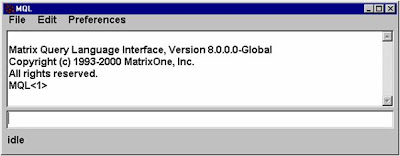
\includegraphics{img/mqlEditor.jpg} \end{center}

\clearpage

\subsubsection*{MQL Help\markboth{MQL Help}{MQL Help}}
\addcontentsline{toc}{subsubsection}{MQL Help}

Execute the below commands for help in MQL-~\\
\begin{itemize}
	\item[] \emph{help;}
	\begin{itemize}
		\item displays general help information
	\end{itemize}
	\item[] \emph{help all;}
	\begin{itemize}
		\item displays entire content of the help file.
	\end{itemize}
	\item[] \emph{help MQL category;}
	\begin{itemize}
		\item displays information about a MQL Category like Type, association, relationship, context, etc and a list of all the statements associated with the category along with the valid syntax.
	\end{itemize}
	\item[] \emph{verbose [on/off];}
	\begin{itemize}
		\item when set to ON, more message detail is provided. When set to OFF, only errors and important system messages are displayed.
	\end{itemize}
\end{itemize}~\\

\begin{center} 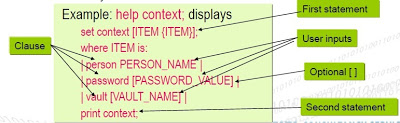
\includegraphics{img/mqlTable.jpg} \end{center} 

\subsubsection*{Context\markboth{Context}{Context}}
\addcontentsline{toc}{subsubsection}{Context}

MQL commands require a person context to access business objects.  ~\\

\begin{itemize}
	\item[] \emph{set context user creator pass ***** vault abc;}
\end{itemize}

\subsubsection*{Quit\markboth{Quit}{Quit}}
\addcontentsline{toc}{subsubsection}{Quit}

Quit statement exits the Matrix command interface and returns control to the operating system. -quit; ~\\

\subsubsection*{MQL Command Abbreviation\markboth{MQL Command Abbreviation}{MQL Command Abbreviation}}
\addcontentsline{toc}{subsubsection}{MQL Command Abbreviation}

Most keywords can be abbreviated to three characters or the least number that will make them unique.  ~\\
\begin{itemize}
	\item[] \emph{help businessobject;}
	\item[] \emph{help bus;}
\end{itemize}

\subsubsection*{Comments\markboth{Comments}{Comments}}
\addcontentsline{toc}{subsubsection}{Comments}

Text appearing after a pound sign (\#), up to and including the next newline, is ignored as a comment.

\begin{itemize}
	\item[] \emph{\#This is a comment line}
	\item[] \emph{list bus; \#list business objects}
\end{itemize} 

\clearpage

\subsubsection*{Name and Value Quotation\markboth{Name and Value Quotation}{Name and Value Quotation}}
\addcontentsline{toc}{subsubsection}{Name and Value Quotation}

Names and values must be quoted (" or ') when they have embedded blanks, tabs, newlines, commas, semicolons, or pound(\#) signs. ~\\

\begin{itemize}
	\item[] \emph{add type Hard Disk; \# Invalid}
	\item[] \emph{add type "Hard Disk"; \# Valid}
	\item[] \emph{add type Memory; \# Valid} ~\\
	Avoid single quotes, double quotes, or commas within names and values.
	\item[] \emph{quote [on/off];} ~\\
	Data strings with embedded spaces are automatically returned as quoted by Matrix. 
\end{itemize}

\subsubsection*{Context\markboth{TCL Mode}{TCL Mode}}
\addcontentsline{toc}{subsubsection}{TCL Mode}

To enter Tcl mode use the command: tcl; ~\\

The command editor prompt will change to: \% ~\\

To exit Tcl mode enter the command: exit; %% ~\\

\subsubsection*{Executing Script \markboth{Executing Script }{Executing Script }}
\addcontentsline{toc}{subsubsection}{Executing Script }

\textbf{\textbf{Syntax:}} \emph{RUN filename;} ~\\
Scripts are created using an ASCII text editor and contain one or more MQL commands ~\\
\textbf{\textbf{Example:}} \emph{RUN "c:/class files/myfile.mql";}

\subsubsection*{Identifying Business Object\markboth{Identifying Business Object}{Identifying Business Object}}
\addcontentsline{toc}{subsubsection}{Identifying Business Object}

Business object have Type, name and revision. You can identify the business objects by its type, name, and revision or by its id . Business Object ID (OID) is a unique identifier for each object. It is defined internally by enovia at a time of object creation. ID of an object can be a substituted for Type, Name, Revision in most MQL commands. It is a unique number of an object across the vault. ~\\ 

\textbf{\textbf{Example:}} by TNR-->Part, S-001,A by id-->20432.14426.20439.1646 %% ~\\

\section*{Extract Information of business objects\markboth{Extract Information of business objects}{Extract Information of business objects}}
\addcontentsline{toc}{section}{Extract Information of business objects}

\subsection*{Listing business object\markboth{Listing business object}{Listing business object}}
\addcontentsline{toc}{subsection}{Listing business object}

	\emph{list businessobject [vault vaultname]}

\subsection*{Listing Admin Object object\markboth{Listing Admin Object object}{Listing Admin Object object}}
\addcontentsline{toc}{subsection}{Listing Admin Object object}

\textbf{\textbf{Syntax:}}
\begin{itemize}
	\item[] \emph{list admintype pattern}
	\begin{itemize}
		\item[] \emph{[select FIELDS]}
		\item[] \emph{[dump [SEPARATOR]]}
		\item[] \emph{[recordsep SEPARATOR]}
	\end{itemize}
\end{itemize} ~\\

\textbf{\textbf{Example:}} List part in vault\_name; (where vault name is optional);
\begin{itemize}
	\item[] \emph{list person;}
	\item[] \emph{list group * select person;}
	\item[] \emph{list policy Pr* select format dump;}
	\item[] \emph{list role * select name assignment dump | recordsep \@;}
\end{itemize}

\clearpage

\subsection*{Printing Business Object or Admin object\markboth{Printing Business Object or Admin object}{Printing Business Object or Admin object}}
\addcontentsline{toc}{subsection}{Printing Business Object or Admin object}

\textbf{Retrieve information about a \underline{single} business or admin object. }~\\
For Admin Object: \emph{Print admin\_object;}~\\
\textbf{\textbf{Syntax:}}
\begin{itemize}
	\item[] \emph{print adminitem NAME}
	\item[] \emph{[selected|select [FIELDs]]}
	\item[] \emph{[dump [SEPARATOR]]}
	\item[] \emph{[output FILENAME];}
\end{itemize}~\\

For Business Object: \emph{print bus bus\_type name revision;} Where, bus\_type name and revision is the type name and revision of the business object. You can substitute Type name and revision by id of the object. ~\\
\textbf{\textbf{Syntax:}}
\begin{itemize}
	\item[] \emph{print businessobject BO\_NAME}
	\begin{itemize}
		\item[] \emph{[selected|select [FIELDs]]}
		\item[] \emph{[dump [SEPARATOR]]}
		\item[] \emph{[output FILENAME];}
	\end{itemize}
\end{itemize}~\\
 
\textbf{Examples:}
\begin{itemize}
	\item[] \emph{print role Sales;}
	\item[] \emph{print type "Hard Disk";}
	\item[] \emph{print format WORD;}
	\item[] \emph{print context;}
	\item[] \emph{print bus 5181.64006.31833.46098;}
	\item[] \emph{print person Dave;}
	\item[] \emph{print bus Monitor NEC A;}
\end{itemize}

\subsection*{Select Clause\markboth{Select Clause}{Select Clause}}
\addcontentsline{toc}{subsection}{Select Clause}

Used to retrieve specific information from Admin Objects, Business Objects, Sets and Connections. ~\\
It can be used in-
\begin{itemize}
	\item Listing Admin Objects
	\item Printing an Admin or Business Object
	\item Printing a Connection
	\item Printing a Set
	\item Expanding a Business Object
	\item Expanding a Set
\end{itemize}~\\

\textbf{\textbf{Example:}}
Specify the field name(s) to be selected
\begin{itemize}
	\item[] \emph{print bus Keyboard "Acme 101" A select attribute;}
	\item[] \emph{print bus Keyboard "Acme 101" A select attribute[Cost];}
	\item[] \emph{print bus Monitor VisionQuest B select id;}
	\item[] \emph{print role select person dump;}
	\item[] \emph{print type Monitor select derived;}
	\item[] \emph{print person select name phone;}
\end{itemize}

\subsubsection*{Dump Clause\markboth{Dump Clause}{Dump Clause}}
\addcontentsline{toc}{subsubsection}{Dump Clause}

Dump clause supress output of field names. Only value(s) with optional separator returned from statement.
\begin{itemize}
	\item[] \emph{print bus Mouse jerry A select attribute[Cost] attribute[size] dump |;}
	\item[] \emph{print bus Monitor NEC A select owner dump;}
\end{itemize} 

\clearpage

\subsubsection*{Output clause \markboth{Output clause }{Output clause }}
\addcontentsline{toc}{subsubsection}{Output clause }

Output clause print the output to a file instead of printing on the console. ASCII text file is created with results of the command.
\begin{itemize}
	\item[] \emph{print bus Note 1000 1 output "c:/notes/1.txt";}
\end{itemize}


\subsection*{Expand\markboth{Expand}{Expand}}
\addcontentsline{toc}{subsection}{Expand}

\begin{itemize}
	\item Used to view connected business objects from a starting object.
	\item Lists the objects that lead to an object, from it, meet selected criteria, or are of a specific type.
	\item Results can be placed into/onto a set or to a file.
	\item Allows the select clause on connected business object or the relationship which links them.
\end{itemize}

\textbf{\textbf{Syntax:}}
\begin{itemize}
	\item[] \emph{expand businessobject BO\_NAME}
	\begin{itemize}
		\item[] \emph{[to|from]}
		\item[] \emph{[relationship PATTERN]}
		\item[] \emph{[type PATTERN]}
		\item[] \emph{[recurse to [all|N]]}
		\item[] \emph{[select businessobject FIELDs]}
		\item[] \emph{[select relationship FIELDs]}
		\item[] \emph{[into|onto set SETNAME]}
		\item[] \emph{[dump [CHAR] [recordsep CHAR]]}
		\item[] \emph{[output FILENAME]}
		\item[] \emph{[terse]}
		\item[] \emph{[limit N];}
	\end{itemize}
\end{itemize}~\\
 
\begin{itemize}
	\item[] \textbf{to|from}
	\begin{itemize}
		\item Specify direction to expand from or to starting object
	\end{itemize}
	\item[] \textbf{relationship, type}
	\begin{itemize}
		\item Filters returned list based on pattern
	\end{itemize}
	\item[] \textbf{recurse}
	\begin{itemize}
		\item Expands connected objects at deeper levels
	\end{itemize}
	\item[] \textbf{select businessobject}
	\begin{itemize}
		\item Selects fields from connected objects
	\end{itemize}
	\item[] \textbf{select relationship}
	\begin{itemize}
		\item Selects fields from connecting relationships
	\end{itemize}
	\item[] \textbf{into|onto set}
	\begin{itemize}
		\item Replaces are appends objects to a set
	\end{itemize}
	\item[] \textbf{dump}
	\begin{itemize}
		\item Removes field information only returning values with optional separator
	\end{itemize}
	\item[] \textbf{recordseparator}
	\begin{itemize}
		\item Replaces default end of record newline ($\backslash$n) with optional chars
	\end{itemize}
	\item[] \textbf{output}
	\begin{itemize}
		\item Output objects to a file
	\end{itemize}
	\item[] \textbf{terse}
	\begin{itemize}
		\item Output object Ids instead of Type, Name, Revision
	\end{itemize}
	\item[] \textbf{limit}
	\begin{itemize}
		\item Limit output to number objects specified
	\end{itemize}
\end{itemize}

\clearpage

\subsection*{Query\markboth{Query}{Query}}
\addcontentsline{toc}{subsection}{Query} 

\begin{itemize}
	\item A query is a search of the Matrix database for objects that meet specified criteria.
	\item Queries are defined, named and saved to the database based on the current context
	\item To produce results queries must be evaluated
	\item Temporary queries are not saved to the database and are evaluated immediately
	%% \item Using .finder to help build complex queries. 
\end{itemize}

\subsubsection*{Add/evaluate query\markboth{Add/evaluate query}{Add/evaluate query}}
\addcontentsline{toc}{subsubsection}{Add/evaluate query}

\textbf{\textbf{Syntax:}}
\begin{itemize}
	\item[] \emph{add query QUERY-NAME}
	\begin{itemize}
		\item[] \emph{[businessobject TYPE* NAME* REV*]}
		\item[] \emph{[owner USER-NAME]}
		\item[] \emph{[vault VAULT-NAME]}
		\item[] \emph{[where QUERY-EXPR];}
		\item[] \emph{evaluate query QUERY-NAME}
		\item[] \emph{[over set NAME]}
		\item[] \emph{[into|onto set NAME]}
		\item[] \emph{[limit VALUE];}
	\end{itemize}
\end{itemize}

\textbf {\textbf{Example:}}

\emph{add query "Find Monitors" bus Monitor * * where 'current == "Planned"';}
\begin{itemize}
	\item New query is added to the database
	\item To retrieve results: \emph{evaluate query "Find Monitors";}
\end{itemize}

\textbf{\textbf{Example:}}
\begin{itemize}
	\item[] \emph{add query "Active NEC Components"}
	\begin{itemize}
		\item[] \emph{businessobject COMPONENT * *}
		\item[] \emph{where 'current == "Active"}
		\item[] \emph{\&\& attribute[Source] == "NEC"';}
	\end{itemize}
\end{itemize}

\textbf{Results:}~\\
Find all the "Component" objects that are in the "Active" state of their policy and have a value of "NEC" for their "Source" attribute. 

\subsubsection*{Temp query\markboth{Temp query}{Temp query}}
\addcontentsline{toc}{subsubsection}{Temp query}

\textbf{\textbf{Syntax:}}
\begin{itemize}
	\item[] \emph{temporary query businessobject TYPE* NAME* REV*}
	\begin{itemize}
		\item[] \emph{[!expand]}
		\item[] \emph{[vault VAULT-NAME]}
		\item[] \emph{[owner USER-NAME]}
		\item[] \emph{[limit VALUE]}
		\item[] \emph{[where]}
		\item[] \emph{[select]}
		\item[] \emph{[dump [CHAR] [recordsep CHAR]]}
		\item[] \emph{[output FILENAME];}
	\end{itemize}
\end{itemize}
 
\textbf{Examples:}
\begin{itemize}
	\item[] \emph{temp query bus Keyboard * *}
	\begin{itemize}
		\item[] \emph{where 'attribute[Cost] < 75';}
	\end{itemize}
	\item[] \emph{temp query bus * * *}
	\begin{itemize}
		\item[] \emph{where 'attribute[Weight] > 0'}
		\item[] \emph{select attribute[Weight]}
		\item[] \emph{attribute[Cost] dump |;}
 	\end{itemize}
	\item[] \emph{temp query bus * * * limit 50;}
	\item[] \emph{temp query bus Mouse * * select attribute[Cost] dump | recordsep \&;}
\end{itemize}

%% \subsubsection*{.finder\markboth{.finder}{.finder}}
%% \addcontentsline{toc}{subsubsection}{.finder}
%% 
%% The last query created in the Matrix application Find
%% \begin{itemize}
%% 	\item Useful for creating complex where clauses
%% 	\item Examining .finder: \emph{print query .finder;}
%% \end{itemize}

\clearpage

\subsection*{Evaluate expression\markboth{Evaluate expression}{Evaluate expression}}
\addcontentsline{toc}{subsection}{Evaluate expression}

Expressions can execute against a collection of business objects, a single business object or a single connection.
\begin{itemize}
	\item[] \emph{evaluate expression EXPRESSION {EXPRESSION}...}
	\begin{itemize}
		\item[] \emph{on {COLLECTION} {BUS OBJECT} {CONNECTION}}
		\item[] \emph{[dump [CHAR]]}
		\item[] \emph{[recordseparator SEPARATOR];}
	\end{itemize}
\end{itemize}~\\

\begin{minipage}[ht]{0.48\textwidth}

	\textbf{Aggregate EXPRESSIONS:}
	\begin{itemize}
		\item count (argument)
		\item sum (argument)
		\item maximum (argument)
		\item minimum (argument)
		\item average (argument)
		\item median (argument)
		\item standarddeviation   (argument)
		\item correlation (cor) (arguments)
	\end{itemize}~\\

\end{minipage} \hfill \begin{minipage}[ht]{0.48\textwidth}

	\textbf{Conditional EXPRESSIONS:}
	\begin{itemize}
		\item if <TEST> then <RESULT> else <RESULT1>
		\item[] \textbf{String expressions}
		\item substring start end text-field
		\item Plus (+) text-field concatenator
	\end{itemize}~\\
	 
	\textbf{Date/Time EXPRESSIONS:}
	\begin{itemize}
		\item MX\_CURRENT\_TIME
	\end{itemize}~\\

\end{minipage}~\\

\textbf{Evaluate expression}
\begin{itemize}
	\item[] \textbf{Valid Business Object COLLECTIONS:}
	\begin{itemize}
		\item set
		\item query
		\item expand
	\end{itemize}
	\item[] \textbf{Collections can be linked:}
	\begin{itemize}
		\item and: object is in both collections
		\item or: object is in one of the collections
		\item less: object in left hand collection only
	\end{itemize}
\end{itemize}~\\
		
\textbf{Examples:}
\begin{itemize}
	\item[] \emph{evaluate expression "count TRUE" on temp query bus "Mon*" * *;}
	\item[] \emph{evaluate expression "count (attribute[Cost] > 0)" on set MySet;}
	\item[] \emph{evaluate expression "sum attribute[Cost]" on expand  Micro Metro0001 A from;}
	\item[] \emph{evaluate expression "count TRUE" on temp query bus * * * less temp query bus Mon* * *;}
	\item[] \emph{evaluate expression "if (count TRUE > 500) then 'Result too big' else 'OK'" on temp query bus * * *;}
	\item[] \emph{evaluate expression "'Owner is:' + owner" on bus Note Metro0001 A;}
	\item[] \emph{eval expression "substring 1 5 Description" on bus Disk Acme A;}
	\item[] \emph{eval expr "(MX\_CURRENT\_TIME - modified)/(3600 * 24)" on bus Note A 1;}
	\item[] \emph{eval expr "(MX\_CURRENT\_TIME - originated)/(3600 * 24) on bus Keyboard Standard A;}
\end{itemize}

\subsection*{Add\markboth{Add}{Add}}
\addcontentsline{toc}{subsection}{Add}

\emph{add object;} Where object should be person, role etc. ~\\
 
\textbf{Syntax:}
\begin{itemize}
	\item[] \emph{add businessobject TYPE NAME REVISION}
	\begin{itemize}
		\item[] \emph{[description DESCRIPTION]}
		\item[] \emph{policy POLICY}
		\item[] \emph{[vault VAULTNAME]}
		\item[] \emph{[ATTRIBUTENAME VALUE];}
	\end{itemize}
\end{itemize}~\\
    
\textbf{Example:}
\begin{itemize}
	\item[] \emph{add bus Keyboard Qwerty A description "Std Keyboard" policy Production Cost 200 Weight .5;}
\end{itemize}

\clearpage

\subsection*{Copy Business Object\markboth{Copy Business Object}{Copy Business Object}}
\addcontentsline{toc}{subsection}{Copy Business Object}

\textbf{Syntax:}
\begin{itemize}
	\item[] \emph{copy businessobject BO\_NAME to NAME REVISION [ITEM {ITEM}];}
\end{itemize}~\\

\textbf{Example:}
\begin{itemize}
	\item[] \emph{copy bus Keyboard Qwerty A to "101 Keys" A owner Ni;}
\end{itemize}~\\

\subsection*{Delete Business Object\markboth{Delete Business Object}{Delete Business Object}}
\addcontentsline{toc}{subsection}{Delete Business Object}

\textbf{Syntax:}		\emph{delete bus BO\_NAME;}~\\

\textbf{Example:}
\begin{itemize}
	\item[] \emph{delete bus Keyboard Standard A;}
	\item[] \emph{delete bus 45181.64006.45205.1092}
\end{itemize}

\subsection*{Modify Business Object\markboth{Modify Business Object}{Modify Business Object}}
\addcontentsline{toc}{subsection}{Modify Business Object}

\textbf{Syntax:}
\begin{itemize}
	\item[] \emph{modify bus BO\_NAME}
	\begin{itemize}
		\item[] \emph{[MODIFY\_ITEM value];}
	\end{itemize}
\end{itemize}~\\
		
\textbf{Example:}
\begin{itemize}
	\item[] \emph{modify bus Mouse A123 A Cost 100 Weight .05;}
	\begin{itemize}
		\item[] \emph{modify bus 20432.14426.20439.27960 owner Dave;}
	\end{itemize}
\end{itemize}

\subsection*{Connect Objects\markboth{Connect Objects}{Connect Objects}}
\addcontentsline{toc}{subsection}{Connect Objects}

\textbf{Syntax:}
\begin{itemize}
	\item[] \emph{connect bus BO\_NAME relationship RELATIONSHIP\_NAME}
	\begin{itemize}
		\item[] \emph{[to|from] BO\_NAME [ATTRIBUTE\_NAME VALUE...];}
	\end{itemize}
\end{itemize}~\\

\textbf{Example:}
\begin{itemize}
	\item[] \emph{connect bus "System Box" "Metro0001" C relationship Assembly to "Hard Disk" Maxtor 3 Quantity 1;}
\end{itemize}

\subsection*{Object Lifecycle Demote/Promote\markboth{Object Lifecycle Demote/Promote}{Object Lifecycle Demote/Promote}}
\addcontentsline{toc}{subsection}{Object Lifecycle Demote/Promote}

\textbf{Syntax:}	\emph{promote bus BO\_NAME;} ~\\

\textbf{Example:}	\emph{promote bus Order 23422 1;} ~\\

~\\

\textbf{Syntax:}	\emph{demote bus BO\_NAME;} ~\\

\textbf{Example:}	\emph{demote bus Order 23422 1;} ~\\


%% \subsection*{MatrixQueryLanguage\markboth{MatrixQueryLanguage}{MatrixQueryLanguage}}
%% \addcontentsline{toc}{subsection}{MatrixQueryLanguage}

\clearpage

%% \section*{Bibliographie\markboth{Bibliographie}{Bibliographie}}
%% \addcontentsline{toc}{section}{Bibliographie}
%% \nocite{*}
%% %toutes references biblio : 6 lettres + 2 chiffres
%% \bibliography{document}
%% \bibliographystyle{frplain} % plain or frplain

\end{document}
